%%%%%%%%%%%%%%%%%%%%%%%%%%%%%%%%%%%%

\section{2.1. Definindo probabilidade}

%%%%%%%%%%%%%%%%%%%%%%%%%%%%%%%%%%%%

\subsection{Probabilidade}

%%%%%%%%%%%%%%%%%%%%%%%%%%%%%%%%%%%%

\begin{frame}
\frametitle{Processos aleatórios}

\twocol{0.5}{0.5}
{
\begin{itemize}
\justifying
\item Num \hl{processo aleatório} sabemos quais resultados \hl{podem acontecer}, mas não sabemos qual resultado específico \hl{irá acontecer}.

\end{itemize}
}{
\begin{center}
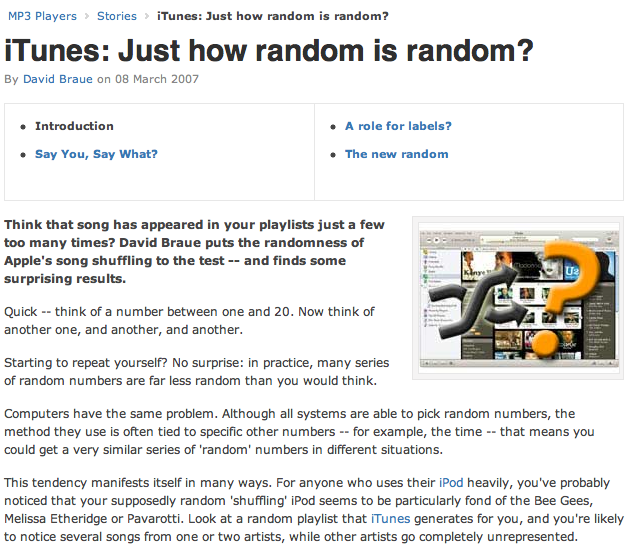
\includegraphics[width=\textwidth]{2-1_define_probability/iTunes.png}
\end{center}
\justifying
\ct{ \webURL{http://www.cnet.com.au/itunes-just-how-random-is-random-339274094.htm}}
}

\end{frame}
%%%%%%%%%%%%%%%%%%%%%%%%%%%%%%%%%%%%

\begin{frame}
\frametitle{Processos aleatórios, tradução do texto}

\justifying
\hl{iTunes: Apenas como aleatório é aleatório?}\\
\vspace{0.5cm}
\justifying
\tiny{
Acha que essa música apareceu nas suas listas de reprodução apenas algumas vezes? David Braue coloca à prova a aleatoriedade do embaralhamento de músicas da Apple - e encontra alguns resultados surpreendentes.\\
\vspace{0.1cm}
\justifying
Por David Braue 4 de agosto de 2008 20:54 AEST\\
\vspace{0.1cm}

\justifying
Rápido - pense em um número entre um e 20. Agora pense em outro, e outro, e outro.\\

\justifying
Começando a se repetir? Nenhuma surpresa: na prática, muitas séries de números aleatórios são muito menos aleatórias do que você imagina.\\
\justifying
Computadores têm o mesmo problema. Embora todos os sistemas sejam capazes de escolher números aleatórios, o método que eles usam é frequentemente vinculado a outros números específicos - por exemplo, o tempo - o que significa que você pode obter uma série muito semelhante de números "aleatórios" em diferentes situações.\\

\justifying
Essa tendência se manifesta de várias maneiras. Para qualquer um que usa streaming de música, provavelmente notou que o “aleatório”, supostamente aleatório, parece gostar particularmente dos Bee Gees, Melissa Etheridge ou Pavarotti. Olhe para uma lista de reprodução aleatória que o iTunes gera para você, e você provavelmente notará várias músicas de um ou dois artistas, enquanto outros artistas ficarão completamente sem representação.
}
\end{frame}
%%%%%%%%%%%%%%%%%%%%%%%%%%%%%%%%%%%%

\begin{frame}
\frametitle{Processos aleatórios (cont.)}

\begin{itemize}
\justifying
\item Exemplos: lançamentos de moedas, lançamentos de dados, iTunes aleatório, se o mercado de ações subir ou descer amanhã, etc.
\justifying
\item Pode ser útil modelar um processo como aleatório, mesmo que não seja verdadeiramente aleatório.

\end{itemize}
\end{frame}

%%%%%%%%%%%%%%%%%%%%%%%%%%%%%%%%%%%%

\subsection{Definindo probabilidade}

%%%%%%%%%%%%%%%%%%%%%%%%%%%%%%%%%%%%

\begin{frame}
\frametitle{Probabilidade}

\begin{itemize}
\justifying
\item Apesar de existirem diferentes interpretações possíveis de probabilidade, elas concordam  com as regras matemáticas que a probabilidade deve seguir.
\begin{itemize}
\item $P(A)$ = Probabilidade do evento A
\item $0 \le P(A) \le 1$
\end{itemize}

\pause
\justifying
\item \hl{Interpretação Frequentista:} 
\begin{itemize}
\justifying
\item A probabilidade de um resultado é a proporção de vezes que o resultado ocorreria se observássemos o processo aleatório um número infinito de vezes.
\end{itemize}
\end{itemize}

\pause
\end{frame}
%%%%%%%%%%%%%%%%%%%%%%%%%%%%%%%%%%%%

\begin{frame}
\frametitle{Probabilidade}

\begin{itemize}
\justifying
\item \hl{Interpretação Bayesiana:} 
\begin{itemize}
\justifying
\item  Um bayesiano interpreta probabilidade como um grau subjetivo de crença: para o mesmo evento, duas pessoas separadas poderiam ter pontos de vista diferentes e, assim, atribuir probabilidades diferentes.
\justifying
\item Amplamente popularizado pelo avanço revolucionário em métodos computacionais e tecnologia.
\end{itemize}

\end{itemize}

\end{frame}

%%%%%%%%%%%%%%%%%%%%%%%%%%%%%%%%%%%%

\begin{frame}
\frametitle{Prática}
\frametitle{Prática}
\justifying
\pq{Você se surpreenderia mais com qual dos seguintes eventos?}

\begin{enumerate}[(a)]
\justifying
\item exatamente 3 coroas em 10 lançamentos de uma moeda.
\justifying
\item exatamente 3 coroas em 100 lançamentos consecutivos de uma moeda.
\justifying
\solnMult{exatamente 3 coroas em 1000 lançamentos consecutivos de uma moeda.}
\end{enumerate}

\end{frame}

%%%%%%%%%%%%%%%%%%%%%%%%%%%%%%%%%%%%

\begin{frame}
\frametitle{Lei dos grandes números}
\justifying
\hl{Lei de grandes números} afirma que à medida que mais observações são coletadas, a proporção de ocorrências de um determinado resultado, \mathhl {\hat {p} _n}, converge para a probabilidade desse resultado, \mathhl {p}.

\end{frame}

%%%%%%%%%%%%%%%%%%%%%%%%%%%%%%%%%%%%

\begin{frame}
\frametitle{Lei dos grandes números (cont.)}
\justifying
\dq{Imagine que em lançamentos consecutivos de uma uma moeda \textit{não viciada}, apareçam cara nos 10 primeiros arremessos. Você apostaria que a chance de aparecer cara no próximo lance é? 0,5, menor que 0,5 ou maior que 0,5?}
\[ \underline{H} \hspace{1mm} \underline{H} \hspace{1mm} \underline{H} \hspace{1mm} \underline{H} \hspace{1mm} \underline{H} \hspace{1mm} \underline{H} \hspace{1mm} \underline{H} \hspace{1mm} \underline{H} \hspace{1mm} \underline{H} \hspace{1mm} \underline{H} \hspace{1mm} \underline{?} \]
\small{
\begin{itemize}
\justifying
\item<2-> A probabilidade ainda é de 0,5, ou seja, ainda há 50\% de chance de que outra cara apareça no próximo lançamento.
\[ P(H \text{ em 11}^{0} \text{ sorteio}) = P(T \text{ em 11}^{0} \text{ sorteio}) = 0.5 \]
\end{itemize}
}
\end{frame}
%%%%%%%%%%%%%%%%%%%%%%%%%%%%%%%%%%%%

\begin{frame}
\frametitle{Lei de grandes números (cont.)}
\justifying

\begin{itemize}
\item  A moeda não  "lembra" o que aconteceu, ela não é influenciada pela quantidade de caras observadas.
\justifying
\item Uma interpretação equivocada da Lei dos Grandes Números é que processos aleatórios devem compensar o que aconteceu no passado; isso não é verdade, essa idéia incorreta é conhecida como \hl{falácia do jogador}.
\end{itemize}

\end{frame}

%%%%%%%%%%%%%%%%%%%%%%%%%%%%%%%%%%%%

\subsection{Mutuamente exclusivos}

%%%%%%%%%%%%%%%%%%%%%%%%%%%%%%%%%%%%

\begin{frame}
\frametitle{Eventos disjuntos}
\justifying
\hl{Eventos disjuntos:} Não podem acontecer ao mesmo tempo.
\begin{itemize}
\justifying
\item O resultado de um único lançamento da moeda não pode ser uma cara e uma coroa ao mesmo tempo.
\justifying
\item Um aluno não pode reprovar e ser aprovado em uma disciplina.
\justifying
\item Uma única carta tirada de um baralho não pode ser um ás e uma dama.
\justifying
\item O resultado de um exame não pode ser positivo \hl{e} negativo.
\justifying
\item A cor de um carro, pode apresentar vários resultados, todos disjuntos.
\end{itemize}

\pause
\justifying
\hl{Eventos não disjuntos:} Podem acontecer ao mesmo tempo.
\begin{itemize}
\justifying
\item Um estudante pode obter um conceito A em Estatística e A em Física no mesmo semestre.
\end{itemize}

\end{frame}

%%%%%%%%%%%%%%%%%%%%%%%%%%%%%%%%%%%%

\begin{frame}
\frametitle{União de eventos}
\justifying
\dq{Qual é a probabilidade de tirar um valete ou uma carta vermelha de um baralho completo bem embaralhado?}

\begin{figure}
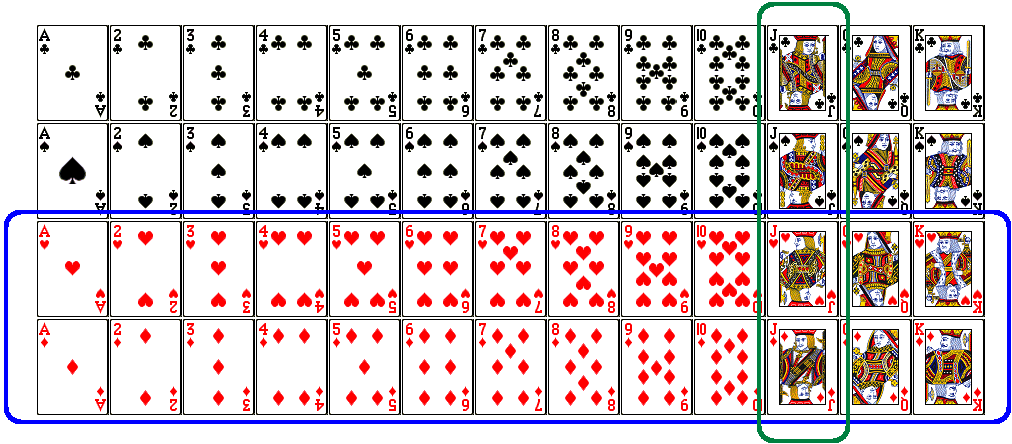
\includegraphics[width=0.7\textwidth]{2-1_define_probability/cards.png}
\end{figure}

\vspace{-0.75cm}

\soln{\onslide<2->{
\begin{align*}
P(valete~ou~vermelho) &= P(valete) + P(vermelho) - \orange{$P(valete~e~vermelho)$} \\
&= \frac{4}{52} + \frac{26}{52} - \frac{2}{52} = \frac{28}{52}
\end{align*}
}}

\vfill

\ct{Figure from \webURL{http://www.milefoot.com/math/discrete/counting/cardfreq.htm}.}

\end{frame}

%%%%%%%%%%%%%%%%%%%%%%%%%%%%%%%%%%%%

\subsection{Probabilidade}

%%%%%%%%%%%%%%%%%%%%%%%%%%%%%%%%%%%%

\begin{frame}
\frametitle{Prática}
\justifying
\pq{Qual a probabilidade de um estudante selecionado aleatoriamente ter a opinião de que a maconha deve ser legalizada \underline{ou} concordar com as opiniões políticas de seus pais?}

{\small
\begin{center}
\begin{tabular}{l  cc c}
            & \multicolumn{2}{c}{\textit{Compartilha a opinião política dos pais}} & \\
\cline{2-3}
\textit{A favor da Legalização} & Não & Sim & Total \\
\hline
Não          & 11 & 40 & 51 \\
Sim         & 36 & 78 & 114 \\
\hline
Total       & 47 & 118 & 165
\end{tabular}
\end{center}
}

\begin{enumerate}[(a)]
\item $\frac{40 + 36 - 78}{165}$
\solnMult{$\frac{114 + 118 - 78}{165}$}
\item $\frac{78}{165}$
\item $\frac{78}{188}$
\item $\frac{11}{47}$
\end{enumerate}

\end{frame}

%%%%%%%%%%%%%%%%%%%%%%%%%%%%%%%%%%%%

\begin{frame}
\frametitle{União de eventos}
\justifying
\formula{Regra da adição}{\[ P(A~ou~B) = P(A) + P(B) - P(A~e~B) \]}
\[ P(A\cup B) = P(A) + P(B) - P(A\cap B) \]
\justifying
\Note{Para eventos disjuntos $P(A~e~B) = 0$, então a fórmula acima será simplificada para $P(A~ou~B) = P(A) + P(B)$.}

\end{frame}

%%%%%%%%%%%%%%%%%%%%%%%%%%%%%%%%%%%%

\subsection{Distribuições de probabilidade}

%%%%%%%%%%%%%%%%%%%%%%%%%%%%%%%%%%%%

\begin{frame}
\frametitle{Distribuição de probabilidade}
\justifying
Uma \hl{distribuição de probabilidade} lista todos os eventos possíveis e as probabilidades com as quais eles ocorrem.

\begin{itemize}
\justifying
\item A distribuição de probabilidade para o resultado do arremesso de uma moeda não viciada:
{\footnotesize 
\begin{center}
\begin{tabular}{r | c | c}
Evento    & Cara (C)		& Coroa (K) \\
\hline
Probabilidade	& 0.5		& 0.5 \\
\end{tabular}
\end{center}
}
\vspace{0.1cm}
\pause
\justifying
\item Regras de uma distribuição de probabilidade:
\begin{enumerate}
\justifying
\item Os eventos listados não podem ocorrer ao mesmo tempo.
\justifying
\item Cada probabilidade deve estar entre 0 e 1.
\justifying
\item As probabilidades somadas devem totalizar 1.
\end{enumerate}

\pause
\justifying
\item A distribuição de probabilidade para o resultado do arremesso de duas moedas:
\soln{
\only<2->{
{\footnotesize
\begin{center}
\begin{tabular}{r | c | c | c | c}
Evento		& CC	& KK		& CK		& KC \\
\hline
Probabilidade	& 0.25	& 0.25	& 0.25	& 0.25 \\
\end{tabular}
\end{center}
}}}

\end{itemize}

\end{frame}

%%%%%%%%%%%%%%%%%%%%%%%%%%%%%%%%%%%%

\begin{frame}
\frametitle{Prática}
\justifying
\pq{Em uma pesquisa, 52\% dos entrevistados disseram que são gremistas. Qual é a probabilidade de que um respondente selecionado aleatoriamente desta amostra seja colorado?}

\begin{enumerate}[(a)]
\justifying
\item 0.48
\justifying
\item mais de 0.48
\justifying
\item menos de 0.48
\justifying
\solnMult{Não pode ser calculada usando apenas a informação dada}\\
\end{enumerate}
\justifying
\soln{\only<2>{\orange{Se há somente dois times, o Grêmio e o Inter, então (a) é possível. No entanto, pode ser que algumas pessoas não torçam pra nenhum time ou que sejam torcedores de outro clube. Então (c) também é possível. A letra (b) não pode ser a resposta, uma vez que a probabilidade seria superior a 1.}}}

\end{frame}

%%%%%%%%%%%%%%%%%%%%%%%%%%%%%%%%%%%%

%%%%%%%%%%%%%%%%%%%%%%%%%%%%%%%%%%%%

\subsection{Complemento de um evento}

%%%%%%%%%%%%%%%%%%%%%%%%%%%%%%%%%%%%

\begin{frame}
\frametitle{Espaço amostral}
\justifying
\hl{Espaço amostral} é a coleção de todos os resultados possíveis de um estudo.

\begin{itemize}
\justifying
\item Um casal tem um filho, qual é o espaço amostral para o sexo da criança? $S = \{ M, F \}$.
\justifying
\item Um casal tem dois filhos, qual é o espaço amostral para o sexo dessas crianças? \soln{\pause{$S = \{ MM, FF, FM, MF \}$}}
\end{itemize}

\pause

\end{frame}
%%%%%%%%%%%%%%%%%%%%%%%%%%%%%%%%%%%%

\begin{frame}
\frametitle{Evento complementar}

\justifying
\hl{Eventos complementares} são dois eventos mutuamente exclusivos cujas probabilidades somam 1.

\begin{itemize}
\justifying
\item Um casal tem um filho. Se sabemos que a criança não é um menino, qual é o sexo dessa criança?
\justifying
\{ \sout{\textcolor{gray}{M}}, \orange{F} \} $\rightarrow$ menino e menina são resultados \hl{complementares}.
\justifying
\item Um casal tem dois filhos, se sabemos que eles não são meninas, quais são as possíveis combinações de gênero para essas crianças?
\soln{\pause{\{ \orange{MM}, \sout{\textcolor{gray}{FF}}, \orange{FM}, \orange{MF} \} }}
\end{itemize}

\end{frame}

%%%%%%%%%%%%%%%%%%%%%%%%%%%%%%%%%%%%

\subsection{Independência}

%%%%%%%%%%%%%%%%%%%%%%%%%%%%%%%%%%%%

\begin{frame}
\frametitle{Independência}
\justifying
Dois processos são \hl{independentes} se o resultado de um não fornecer informações úteis sobre o resultado do outro.

\pause

\begin{itemize}
\justifying
\justifying
\item Sabendo que o resultado do primeiro lançamento da moeda foi cara, \underline{isso não é} uma informação útil para determinar em que lado a moeda cairá no segundo lançamento. $\rightarrow$ Os resultados de dois lançamentos de uma moeda são independentes.

\pause
\justifying
\item Sabendo que a primeira carta tirada de um baralho é um ás, \underline{é fornecida uma informação útil} para determinar a probabilidade da segunda carta ser um ás. $\rightarrow$ Os resultados da seleção (sem reposição) de duas cartas de um baralho são dependentes.

\end{itemize}

\end{frame}

%%%%%%%%%%%%%%%%%%%%%%%%%%%%%%%%%%%%

\begin{frame}
\frametitle{Prática}
\justifying
\pq{\small{Entre os dias 9 e 12 de janeiro de 2013, a SurveyUSA entrevistou uma amostra aleatória de 500 moradores de NC, a pergunta era: permitir a posse de armas protege os cidadãos que respeitam a lei, ou torna a sociedade mais perigosa. 58\% de todos os entrevistados disseram que protege os cidadãos. 67\% dos entrevistados brancos, 28\% dos entrevistados negros e 64\% dos entrevistados hispânicos compartilharam essa visão. Qual das alternativas abaixo é verdadeira?}}
\justifying
A opinião sobre posse de armas e raça/etnia são
\begin{enumerate}[(a)]
\item complementares
\item Mutualmente exclusivas
\item independentes
\solnMult{dependentes}
\item disjuntas
\end{enumerate}
\justifying
\ct{\webURL{http://www.surveyusa.com/client/PollReport.aspx?g=a5f460ef-bba9-484b-8579-1101ea26421b}}

\end{frame}

%%%%%%%%%%%%%%%%%%%%%%%%%%%%%%%%%%%%

\begin{frame}
\frametitle{Prática}
\justifying
\formula{Verificando a independência}{Se P(A ocorre, dado que B é verdade) = $P(A~|~B) = P(A)$, então A e B são independentes.}

$\:$ \\

\soln{\pause{P(protege os cidadãos) = 0.58 \\
\pause
$\:$ \\
\justifying
P(opinião de que posse de armas protege os cidadãos, dado que o residente é branco) = \\ P(protege os cidadãos $|$ branco) = 0.67 \\
$\:$ \\
P(protege os cidadãos $|$ negro) = 0.28 \\
$\:$ \\
P(protege os cidadãos $|$ hispânico) = 0.64 \\
$\:$ \\
\pause
\justifying
P(protege os cidadãos) varia de acordo com a raça/etnia, portanto, a opinião sobre a posse de armas e raça/etnia devem ser dependentes.
}}

\end{frame}

%%%%%%%%%%%%%%%%%%%%%%%%%%%%%%%%%%%%

\begin{frame}
\frametitle{Determinando a dependência com base em dados amostrais}

\begin{itemize}
\justifying
\item Se as probabilidades condicionais calculadas com base nos dados da amostra sugerem dependência entre duas variáveis, o próximo passo é conduzir um teste de hipóteses para determinar se a diferença observada entre as probabilidades é provável ou improvável de ter ocorrido.
\justifying
\item Se a diferença observada entre as probabilidades condicionais for grande, então há evidências mais fortes de que a diferença é real.
\end{itemize}
\end{frame}

%%%%%%%%%%%%%%%%%%%%%%%%%%%%%%%%%%%%

\begin{frame}
\frametitle{Determinando a dependência com base em dados amostrais}

\begin{itemize}
\justifying
\item Se uma amostra é grande, então até mesmo uma pequena diferença pode fornecer forte evidência de uma diferença real.

\end{itemize}

\pause
\justifying
\dq{{\small Vimos que P(protege os cidadãos $|$ branco) = 0.67 e P(protege os cidadãos $|$ hispânico) = 0.64. Sob qual condição você estaria mais convencido de uma diferença real entre as proporções de brancos e hispânicos que acham que a posse de armas protege os cidadãos? $n = 500$ ou $n = 50,000$}} \pause \soln{$n = 50,000$}

\end{frame}

%%%%%%%%%%%%%%%%%%%%%%%%%%%%%%%%%%%%

\begin{frame}
\frametitle{Regra do produto para eventos independentes}
\justifying
\formula{Regra do produto para eventos independentes}{\[P(A~e~B) = P(A) \times P(B) \]
\small{Ou mais geralmente, $P(A_1~e~\cdots~e~A_k) = P(A_1) \times \cdots \times P(A_k)$}}

\pause
\justifying
\dq{Você joga uma moeda duas vezes, qual é a probabilidade de observar duas coroas seguidas?}

\pause
\justifying
\[ P(\text{Coroa no primeiro lance}) \times  P(\text{Coroa no segundo lance}) = \frac{1}{2} \times \frac{1}{2} = \frac{1}{4} \]

\end{frame}

%%%%%%%%%%%%%%%%%%%%%%%%%%%%%%%%%%%%

\begin{frame}
\frametitle{Prática}
\justifying
\pq{Uma pesquisa recente da Gallup sugere que 25,5\% dos texanos não têm plano de saúde, a pesquisa foi realizada em junho de 2012. Supondo que a proporção de pessoas sem seguro permaneça constante, qual é a probabilidade de que dois texanos selecionados aleatoriamente não tenham seguro?}

\twocol{0.4}{0.6}
{
\begin{enumerate}[(a)]
\item $25.5^2$
\solnMult{ $0.255^2$ }
\item $0.255 \times 2$
\item $(1 - 0.255)^2$
\end{enumerate}
}
{
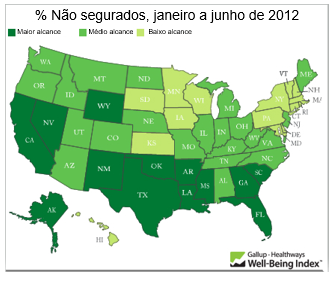
\includegraphics[width=0.9\textwidth]{2-1_define_probability/uninsured.png}
}
\justifying
\ct{ \webURL{http://www.gallup.com/poll/156851/uninsured-rate-stable-across-states-far-2012.aspx}}

\end{frame}

%%%%%%%%%%%%%%%%%%%%%%%%%%%%%%%%%%%%

\subsection{Recapitulando}

%%%%%%%%%%%%%%%%%%%%%%%%%%%%%%%%%%%%

\begin{frame}
\frametitle{Disjuntos vs. complementares}
\justifying
\dq{A soma das probabilidades de dois eventos disjuntos sempre somam 1?}

\pause
\justifying
\soln{Não necessariamente, pode haver mais de dois eventos no espaço amostral, por exemplo, times de futebol.}

\pause
$\:$ \\
\justifying
\dq{A soma das probabilidades de dois eventos complementares sempre somam 1?}

\pause
\justifying
\soln{Sim, essa é a definição de complementar, por exemplo, cara e coroa. }

\end{frame}

%%%%%%%%%%%%%%%%%%%%%%%%%%%%%%%%%%%%

\begin{frame}
\frametitle{Voltando ao exemplo do plano de saúde}
\justifying
\dq{Se fôssemos selecionar aleatoriamente 5 texanos, qual é a probabilidade de que pelo menos um não tenha plano de saúde?}

\begin{itemize}
\justifying
\item Se fôssemos selecionar aleatoriamente 5 texanos, o espaço amostral do número de texanos que não têm seguro seria:
\[ S = \{0, 1, 2, 3, 4, 5\} \]
\justifying
\item Estamos interessados em casos em que pelo menos uma pessoa não tem seguro:
\[ S = \{0, \orange{$1, 2, 3, 4, 5$} \} \]
\justifying
\item Então, podemos dividir o espaço amostral em duas categorias:
\[ S = \{0, \orange{pelo~menos~um} \} \]

\end{itemize}

\end{frame}

%%%%%%%%%%%%%%%%%%%%%%%%%%%%%%%%%%%%

\begin{frame}
\frametitle{Voltando ao exemplo do plano de saúde}
\justifying
A probabilidade do espaço amostral deve totalizar 1:
\begin{eqnarray*}
Prob (pelo~ menos ~ 1 ~ sem ~seguro) &=& 1 - Prob (nenhum ~ sem ~seguro) \\
\pause
&=& 1 - [(1-0.255)^5] \\
\pause
&=& 1- 0.745^5 \\
\pause
&=& 1 - 0.23 \\
\pause
&=& 0.77
\end{eqnarray*}

$\:$ \\
$\:$ \\
\justifying
\formula{Pelo menos 1}{\[P(pelo~ menos ~ um) = 1 - P(Nenhum)\]}

\end{frame}

%%%%%%%%%%%%%%%%%%%%%%%%%%%%%%%%%%%%

\begin{frame}
\frametitle{Prática}
\justifying
\pq{Aproximadamente 20\% dos alunos de graduação são vegetarianos ou veganos. Qual é a probabilidade de que, numa amostra aleatória de 3 universitários, pelo menos um seja vegetariano ou vegano?}

\twocol{0.3}{0.6}{
\begin{enumerate}[(a)]
\item $1 - 0.2 \times 3$
\item $1 - 0.2^3$
\item $0.8^3$
\item $1 - 0.8 \times 3$
\solnMult{$1 - 0.8^3$}
\end{enumerate}
}
{
\soln{ \only<2>{
$P(pelo~menos~1~ser~veg) = 1- P(\textit{não}~veg)$ \\
$= 1 - (1 - 0.2)^3$ \\
$= 1 - 0.8^3$ \\
$= 1 - 0.512 = 0.488$ }}
}

\end{frame}

%%%%%%%%%%%%%%%%%%%%%%%%%%%%%%%%%%%%


